\section{Results}
The results of our experiments were obtained thanks to the ChiVO\footnote{\texttt{https://chivo.cl/}} (Chilean Virtual Observatory) datacenter \citep{solar2015chilean} by using an Intel Xeon CPU E5-2680 2.50GHz with 12 cores and 64 GB of RAM.

\subsection{Number of States Impact}
\begin{table}[!t]
    \caption{Macro averaged F1-score on validation set for different number of settings. $n_{up}$ stands for the number of positive states while $n_{down}$ corresponds to negative states defined for the MTF representation. $*$ symbol shows the best result.}
    \label{tab:exp_states}
    \centering
    \begin{tabular}{c|ccccc}
        \diaghead(-2,1){\hspace{1.7cm}}{$n_{up}$}{$n_{down}$}& %do not change
            8 & 16 & 32 & 64 \\ \hline
        4  & 71.48 & 72.66 & 72.97 & 71.81 \\ 
        8  & 72.14 & 73.35 & 74.43 & 72.00 \\ 
        16 & 72.84 & 74.69 & 75.75$^*$ & 74.13  \\ 
        32 & 73.84 & 75.03 & 75.40 & 75.53 \\  
        64 & 72.75 & 73.47 & 74.03 & 74.95  \\ 
        \hline
        %128 & $\times$ & $\times$ & $\times$ & $\times$ & $\times$ %& Si
    \end{tabular}
\end{table}
Table \ref{tab:exp_states} presents the experimental impact of the number of states in the classification task. 
The best \textit{F1-score} was obtained by using $n_{up} = 16$ and $n_{down}=32$, which is a 2-channel image of $48\times 48$ size.
Note that as the number of states increases (both $n_{up}$ and $n_{down}$), the performance improves, this is because the model input becomes a fine-grained representation (more detailed image).  
However, for any $n_{up}$ up to 16 states, macro averaged \textit{F1-score} reaches a maximum with $n_{down}=32$, then it decays. %(with $n_{down}=64$). 
The experimental results show that the number of transitions does not need a more fine-grained representation ($n_{down} \geq 64$) because the transit information turns fuzzy, so each pixel of the image does not represent aggregated information. In that sense, the MTF image results in a very sparse matrix, since there is a lot of states but only a few transitions per state. 

By using $n_{up}=32$ or $n_{up}=64$, when more $n_{down}$ states are used a higher \textit{F1-score} is reached.
This shows that the positive-negative symmetric states, i.e. $n_{up}=n_{down}$, are not always the best setting.
Most of the cases reach better results when a higher number of states on the negative values is set.
Indeed, given an $n_{up}$, the number of negative states ($n_{down}$) should be higher or equal to $n_{up}$. 
This makes sense if we analyze the problem context since the negative transitions (light blocking) are more important than the positive ones (noise and stellar properties).

\subsection{Method Comparison}
Using the best setting on validation set, $48\times 48$ images ($n_{up} = 16 $ and $n_{down} = 32$), we obtain the final results on the test set against the compared methods.

\begin{table}[!t]
\caption{Classification performance using different methods and feature extraction techniques. The \textit{F1-score} per class (C: \textit{Confirmed}, FP: \textit{False Positive}) and the macro averaged \textit{F1-score} are presented. $\star$ The feets results reported corresponds to a sample of 2500 objects (2 months execution).}
\label{tab:class_results}
\begin{tabular}{c|c|cc|c} \hline
\textbf{Method} & \textbf{Input shape} & \textbf{FP class}& \textbf{C class} & \textbf{Macro avg.} \\ \hline 
\multicolumn{5}{c}{\textit{Specialized hand-crafted features + Classic Learning Methods}} \\ \hline
Metadata  & $10$                 & $90.13$ & $83.85$  & $87.00$ \\ %\hline
feets$^{\star}$     & $57$                 & $84.57$ & $31.19$  & $57.88$    \\ \hline
\multicolumn{5}{c}{\textit{Feature extraction + Classic Learning Methods}} \\ \hline
F-PCA  & $32$                 & $80.03$ & $58.54$  & $69.29$ \\ \hline
%fourier + ica??
\multicolumn{5}{c}{\textit{Deep Learning Methods}} \\ \hline
1D CNN raw  & $70000\times 2$         & $84.43$ & $67.68$ & $76.06$  \\ 
\textbf{2D CNN MTF} 
            & $48\times48\times 2$    & $84.26$   & $69.76$  & $77.01$   \\ 
\hline
%poner folded? yo diria que no .. ya que les va muy bien jaja y enrealidad hacen trampa al conocer el periodo.. (si se sabe el periodo mejor usar la metadata)
\end{tabular}
\end{table}
Table \ref{tab:class_results} compares different methods according to \textit{F1-score} metric.  %remarked in baseline section for the exoplanet detection problem by \textit{F1-score}. 
The classification for classic learning was made using the fully connected block of deep architectures (Table \ref{tab:model:arch}). This corresponds to 128 dense units with \textit{relu} activation function followed by the classification dense layer with one unit and \textit{sigmoid} activation function. 
Firstly, our method obtains a moderate F1-score macro averaged improvement of 0.95 over a 1D CNN, despite of the 1D CNN method uses a fairly sophisticated architecture with a large number of parameters (Table \ref{tab:model:arch}).
Drawing on 2D CNN model, our method extracts enough information to identify transit patterns on the MTF images.

Deep learning methods outperform the classic counterpart approach of F-PCA by $\sim 8\%$ and the hand-crafted features of feets showing a large gap ($\sim 33\%$). 
However, the specialized features for the problem, metadata, have the best performance for the task. 
Note that our method reaches the second best result, meaning that still are some improvements that could be done with the automatic techniques.

The detailed metrics per class show that the confirmed class is the most difficult to detect, meaning that the behavior of the exoplanets is not so clear in order to group and discriminate correctly all the patterns. 
The advantage from the metadata representation comes from this class, showing large improvement against all the other methods. 
The false positive class (non-exoplanets) appears easier to detect, based on the \textit{F1-score} higher than 80\% for all the methods. 
%While the false positives class (non-exoplanets) appears more easier to detect based on the probably clear patterns of the binary system or noise properties.

\begin{table}[!t]
\caption{Time comparison in seconds for different learning techniques. Values in parenthesis on Training column stands for the number of epochs to train the models. $\diamond$ This value is based on the information of \citep{fanelli2011kepler}, this is 4 days. $\star$ The feets representation time is measured over a subset of 2500 objects (30\% of the data).}
\label{tab:time_results}
\begin{tabular}{c|ccc|c} \hline
\textbf{Method} & \textbf{Representation} & \textbf{Training} & \textbf{Predict} & \textbf{Total} \\ \hline 
\multicolumn{5}{c}{\textit{Specialized hand-crafted features + Classic Learning Methods}} \\ \hline
Metadata   & $5760^\diamond$ & $37.8$ (200)  & $0.04$ & - \\ %\hline
feets      & $5912500^{\star}$   & $42.2$ (200)  & $0.07$ & $>100000$ mins \\ \hline %($2365$ x D)
\multicolumn{5}{c}{{\textit{Feature extraction + Classic Learning Methods}}} \\ \hline
F-PCA          & $166.6$  & $40.4$ (200) & $0.06$ & $\sim$ 4 mins \\ \hline  %\hline %$96.6$ (Fou) $0.012$ x D , $70$ (PCA
\multicolumn{5}{c}{{\textit{Deep Learning Methods}}} \\ \hline
1D CNN raw             & $0$ & $21500$ (50)  & $288.33$ & $\sim$ 360 mins  \\ 
\textbf{2D CNN MTF} 
                       & $145$ & $1040$ (200) & $4.72$ & $\sim$ 20 mins \\ %($0.018$ x D)
\hline
\end{tabular}
\end{table}
Table \ref{tab:time_results} shows the execution time by phase: i) the representation of the method, ii) training of the model and iii) predict; The total time is presented too.
Our method takes 20 minutes in average for running the complete process.  This includes the generation of all the MTF images for our dataset, training the 2D CNN model and predict on the test set partition.
This value is reasonable good compared to more specialized methods, such as the use of metadata (more than 4 days\footnote{This value is based on the information of \citep{fanelli2011kepler}} ) or feets features (more than 2 months).
%%%%%% opcion 1
%The execution time of our method becomes close but not faster than the classic method of F-PCA, but since our proposal managed to exceed this method in terms of macro averaged \textit{F1-score} is a reasonable trade-off.
%%% opcion 2
Despite the fact that the execution time of our method does not reach faster results than F-PCA, our method managed to outperform classic methods in terms of macro averaged \textit{F1-score}.

Finally, comparing our method against other deep learning techniques, we can see that our method has a shorter execution time than 1D CNN which uses the raw light curve. Despite 1D CNN method does not need a representation phase, this model has a quite high temporary cost on training and prediction steps due to the more complex processing. Our method focus on the representation but reduce time on training and prediction phases (a simpler model)
That is, using a 2D CNN model we can extract important information in a faster way, 18 times shorter: from 6 hours to just 20 minutes as total execution time.

\section{Interpreting the MTF Image Content}
\begin{figure}[t!]
\centering
    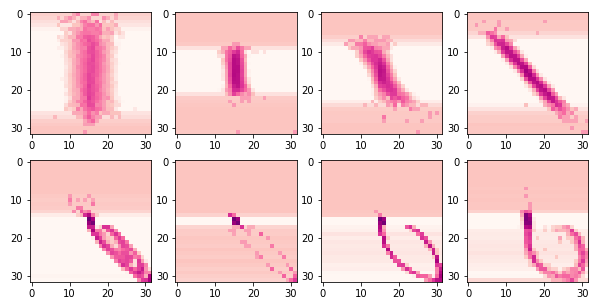
\includegraphics[width=.9\linewidth]{imgs/MTF_LC.png}
\caption{Examples of different types of behavior on MTF of Kepler mission. Only the confirmed objects (exoplanets) are shown here ($32\times 32$ matrix).}
\label{ex:mtf}
\end{figure}
The proposed MTF matrix is useful to illustrate the \textit{global} behavior of all the uneven measurements of light curves in a simpler way, specially if the number of measurements are more than 10 thousand values (as in our case).
The exoplanet transit problem allows us to interpret the light curve transitions channel. For example, the minor state corresponds to the moment when the planet is in front of its host star and blocks the maximum light. While the center state, on positive-negative symmetric matrix, means that the light of the star is measured cleanly (with no eclipsing objects or stellar noise).
 
Figure \ref{ex:mtf} shows different patterns in the transition channel of the MTF images. The objects correspond to confirmed exoplanets light curves of the dataset.
Here, is possible to identify two main types of behavior: diagonal and vertical. Within the diagonal patterns there are two types: ellipse and line, where the latter corresponds to an ellipse with maximum eccentricity ($e=\infty$). 

% + eccentricco + lineal  => lento proceso (periodo alto)
% - eccentrico + ovalado  => rapido proceso (periodo bajo)
The results allow us to discuss the following points.
The diagonal or ellipse patterns are present on those objects whose light curve accounts for clean measurements where eclipses are easily identify. 
Specifically, the level of eccentricity of transitions in MTF is related to the period of the transit object observed on the light curve. 
That is, curves with shorter period (faster transit) show more circular patterns (\textit{smaller eccentricity} on the ellipse) since they have more abrupt transitions between two contiguous points of the time series. 
Instead, a longer period (slower transit) indicates smooth transitions between the states, giving to more diagonal patterns (\textit{high eccentricity}) as observed in Figure \ref{ex:mtf} and Figure \ref{fig:mtf_ex}.
In summary, more eccentricity on the MTF behavior indicates slower orbiting planets.

\begin{figure}[t!]
    \centering
    \subfloat{{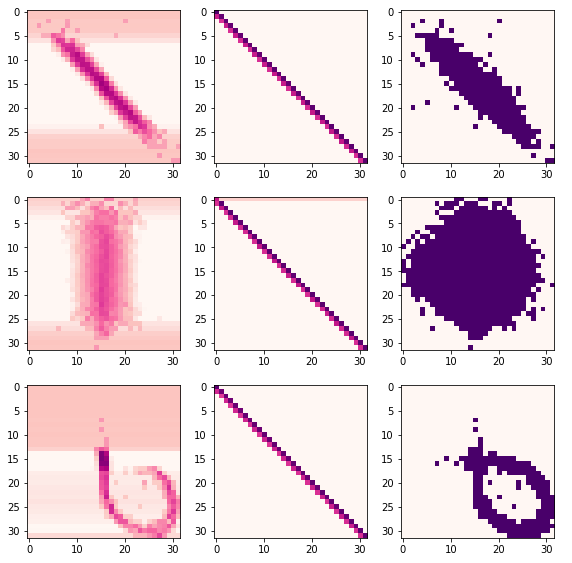
\includegraphics[width=0.45\textwidth]{imgs/Tiny_MTF1.png} }}%
    \qquad
    \subfloat{{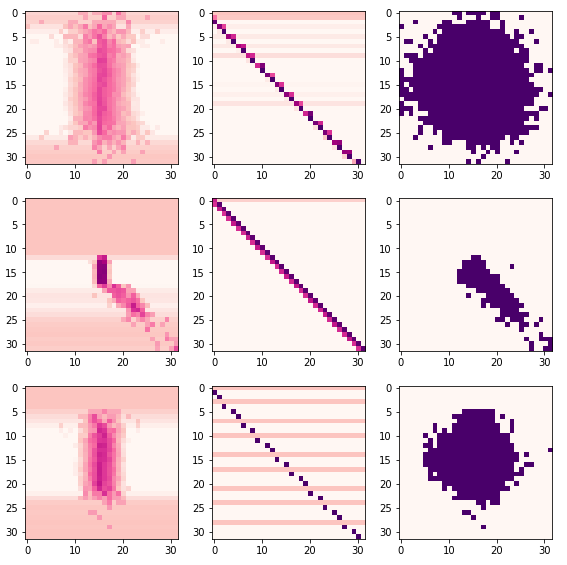
\includegraphics[width=0.45\textwidth]{imgs/Tiny_MTF2.png} }}%
    \caption{Six examples of transition patterns observed on Kepler light curves. In the left is the measurement channel, transitions represented as probabilities (normalized). In the center is the time channel, from the temporal information of the light curve. On the right there is a binarized representation of the measurement channel, 1 if there is a transition between states.}%
    \label{fig:mtf_ex}
\end{figure}
On the other hand, vertical patterns are associated with objects whose light curve presents extremely diffuse transitions. These curves are generally accompanied by a high rate of measurement errors so transitions between states occur \textit{randomly} with the highest concentration at equilibrium states (central zone of the MTF). This phenomenon can be observed in the binary transition images (Figure \ref{fig:mtf_ex}) where there are transitions in almost all the states of the generated MTF. However, when the transitions counts are normalized, vertical patterns are observed.

Note that there are larger behavior patterns that cover the entire range of states. That is, there are measurements near the maximum or minimum value ($1 $ and $- 1$). 
Thus, larger patterns denote a significant number of transitions across the complete spectrum, while shallow patterns denote that the highest concentration of transitions occurs in central states with no focus on extreme values.


\begin{figure}[t!]
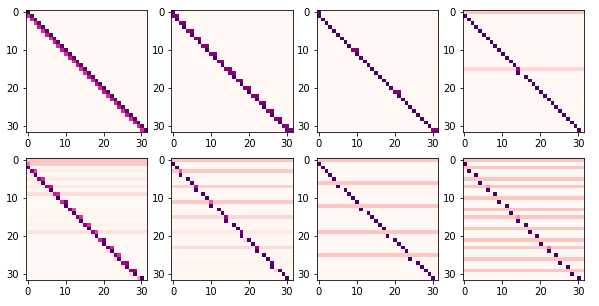
\includegraphics[width=.9\linewidth]{imgs/MTF_Time.png}
\caption{Example of different types of behavior on the time transitions MTF on Kepler mission. Only the confirmed objects (exoplanets) are shown here. $32\times 32$ matrix}
\label{ex:mtf_time}
\end{figure}
Following the analysis for the time channel on the MTF image representation, Figure \ref{ex:mtf_time} shows different observed behavior from confirmed exoplanets on the Kepler mission.
It can be seen that there are some continuous time transitions (exactly diagonal) and others with more discontinuous patterns (diagonal with cuts).
This last one occurs when the light curve transitions have a high delta time that does not meet the specified maximum delta $T_d$, this mean that some sampling rates are greater than the specified by Kepler (half an hour).
The discontinuous patterns are expected because the light curve could have irregularities based on the unevenly-sampled measurements of Kepler dataset, i.e. astronomical phenomenon that obstruct the observation.


\subsection{Model Prediction Analysis}
\begin{figure}[!t]
    \centering
\begin{tabular}{c}
    Confirmed (Exoplanet) predictions (with high confidence) \\
    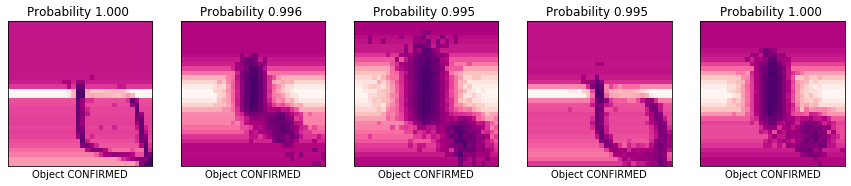
\includegraphics[width=0.95\textwidth]{imgs/MTF_confE_data_v2.png}  \\
    False Positive (Non-Exoplanet) predictions (with high confidence) \\
     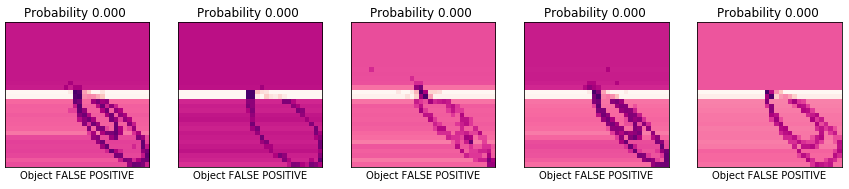
\includegraphics[width=0.95\textwidth]{imgs/MTF_confNE_data_v2.png} \\
    Difficult objects predictions (very low confidence) \\
    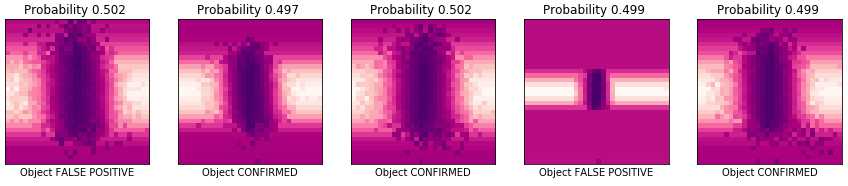
\includegraphics[width=0.95\textwidth]{imgs/MTF_diff_data_v2.png}
\end{tabular}
\caption{Examples on different types of predictions of the KOI objects (MTF).}
\label{fig:mtf_pred_ex}
\end{figure} %cmap es RdPu, sin limite en lognorm (el valor maximo y mas oscuro, no es 1)
Figure \ref{fig:mtf_pred_ex} shows examples of our representation for the KOI objects (MTF) that the 2D CNN model predicts with high reliability. We use the model probability predictions, $p(y=\texttt{confirmed})$, to understand the shape of objects with probability close to 1 (most likely confirmed) and close to 0 (most likely false positive). 

As previously stated, the standard well defined transits (without noise or random behavior) are objects with bottom right ellipse patterns, where the objects predicted as confirmed have more thick pattern than the objects predicted as false positives.
There also seems to be a second ellipse on the false positive objects, meaning perhaps a binary system (two stars eclipsing each other with two statistical different transits). 
These two intrinsic characteristic could be the factors that our model consider in order to classify as a certain class: analyze the type of pattern into the bottom diagonal (\textit{it is clearly only one ellipse?}) and how thick are the patterns.

In addition, we show the most difficult objects to classify, where the model is not sure of the class label (probability close to 0.5).
On this case it can be seen a big spot on the center with no clear inclination to the bottom right. These patterns are the vertical ones commented earlier which we associate to random transitions. 
This clarifies the difficulties of classify these types of objects despite the fact that some of them have an orbiting exoplanet. Therefore, there does not appear to be a clear difference between objects with or without exoplanets.